\documentclass[11pt,letterpaper]{article}
\usepackage[T1]{fontenc}
\usepackage[utf8]{inputenc}
\usepackage{lmodern,microtype}
\usepackage[margin=0.88in,headheight=15pt]{geometry}
\usepackage{amsmath,amssymb,amsthm,mathtools,stmaryrd}
\usepackage{booktabs,longtable,tabularx,array,enumitem}
\usepackage{xcolor,listings,tikz}
\usetikzlibrary{arrows.meta,positioning,fit,backgrounds}
\usepackage[most]{tcolorbox}
\usepackage{fancyhdr,xurl,hyperref,bookmark}
\definecolor{Navy}{HTML}{18354A}
\definecolor{Teal}{HTML}{156A70}
\definecolor{Pale}{HTML}{F2F6F8}
\definecolor{Rule}{HTML}{C9D5DB}
\hypersetup{colorlinks=true,linkcolor=Navy,citecolor=Teal,urlcolor=Teal,
  pdftitle={Leant2: A Lean-Native Architecture for Proof-Carrying Program Synthesis},
  pdfauthor={OpenAI},pdfsubject={Dependent synthesis, behavioral constraints, certified recursion}}
\pagestyle{fancy}\fancyhf{}
\fancyhead[L]{\small Leant2: architecture and algorithms}
\fancyhead[R]{\small 17 September 2026}
\fancyfoot[C]{\thepage}
\setlength{\parskip}{4pt}\setlength{\parindent}{1em}
\emergencystretch=2em
\setlist{itemsep=3pt,topsep=5pt,leftmargin=1.7em}
\newcolumntype{Y}{>{\raggedright\arraybackslash}X}
\newcommand{\code}[1]{\texttt{\detokenize{#1}}}
\newcommand{\Lean}{Lean~4}
\newcommand{\Spec}{\mathsf{Spec}}
\newcommand{\Sat}{\mathsf{Sat}}
\newcommand{\K}{\mathcal K}
\newcommand{\G}{\mathcal G}
\newcommand{\E}{\mathcal E}
\newcommand{\M}{\mathcal M}
\newtheorem{theorem}{Theorem}[section]
\newtheorem{proposition}[theorem]{Proposition}
\newtheorem{lemma}[theorem]{Lemma}
\theoremstyle{definition}\newtheorem{definition}[theorem]{Definition}
\newtheorem{example}[theorem]{Example}
\theoremstyle{remark}\newtheorem{remark}[theorem]{Remark}
\newtcolorbox{designbox}[1]{enhanced,breakable,colback=Pale,colframe=Rule,
  boxrule=0.6pt,arc=1mm,title={#1},coltitle=Navy,colbacktitle=Pale,fonttitle=\bfseries}
\lstdefinelanguage{LeanLike}{morekeywords={import,open,namespace,end,def,theorem,
  inductive,structure,where,match,with,fun,let,in,by,do,return,if,then,else,
  partial,forall,Type,Sort,Prop,exact,intro,constructor,apply,cases,have},
  morecomment=[l]{--},morecomment=[s]{/-}{-/},morestring=[b]"}
\lstset{language=LeanLike,basicstyle=\ttfamily\footnotesize,
 keywordstyle=\bfseries\color{Navy},commentstyle=\color{Teal},
 backgroundcolor=\color{Pale},frame=single,rulecolor=\color{Rule},
 breaklines=true,columns=fullflexible,keepspaces=true,showstringspaces=false,
 aboveskip=8pt,belowskip=8pt,
 literate={→}{{$\to$}}2 {←}{{$\gets$}}2 {∀}{{$\forall$}}1 {×}{{$\times$}}1
 {∧}{{$\land$}}1 {∨}{{$\lor$}}1 {¬}{{$\neg$}}1 {⟨}{{$\langle$}}1 {⟩}{{$\rangle$}}1
 {·}{{$\cdot$}}1 {α}{{$\alpha$}}1 {β}{{$\beta$}}1 {λ}{{$\lambda$}}1
 {∈}{{$\in$}}1 {≤}{{$\le$}}1 {≠}{{$\ne$}}1 {ℕ}{{$\mathbb N$}}1}
\title{\textbf{Leant2: A Lean-Native Architecture\\for Proof-Carrying Program Synthesis}\\[7pt]
\large Dependent types, behavioral constraints, and certified recursion}
\author{Architecture study and executable research prototype}
\date{17 September 2026}
\begin{document}
\maketitle
\begin{abstract}
Leant2 should not be a transliteration of a Haskell synthesizer. It should be a
Lean-native search system whose basic problem is to construct a term together
with a proof of its requested behavior. This article develops that design in
implementation-level detail. Exact Lean expressions, universes, local contexts,
and dictionary values remain authoritative throughout search. A portfolio of
focused introduction, dependent elimination, library application, certified
recursion schemes, finite sketch solving, and proof search operates over
transactional, dependency-aware obligation graphs. A separate admission boundary
checks completed declarations and their dependencies with the Lean kernel.

The central algorithmic choice is to retain the continuation of the entire
program-and-proof problem: solving a value hole does not commit that value before
its remaining behavioral obligations succeed. This prevents a common loss of
solutions in otherwise sound inhabitation search. Additional design rules cover
higher-rank universe instantiation, dependent projections, recursive-call
capabilities, invariant-carrying fold states, counterexample-guided refinement,
reversible observational buckets, and honest negative results. We distinguish
kernel soundness, restricted search completeness, and empirical practical coverage.

The accompanying Lean prototype was remotely compiled with Lean 4.34.0. It passes
21 synthesis examples, four rejection controls, and eight additional statements.
Twenty-four of its 25 audited declarations use no axioms; an indexed elimination
uses only \code{propext}. A separate checked artifact implements proof-carrying
structural recursion and proves a synthesized affine-fold instance correct for
all input lists. Two executable Python models test reversible observational
partitioning and finite sketch selection. These are feasibility experiments, not
an implementation or benchmark of the entire proposed system.
\end{abstract}

\begin{designbox}{Recommendation}
Build an exact-expression synthesis library first, exposed as a Lean tactic and
command. Run that same library in a project-toolchain-matched worker for a REPL
or editor service. Keep all semantic components in Lean; keep search heuristic
and replaceable; make checked terms and explicit evidence the only route to
accepted results. Prioritize dependent elimination and contract-carrying
recursion over another target-neutral type representation.
\end{designbox}
\clearpage
\setcounter{tocdepth}{1}
\tableofcontents
\clearpage

\section{The starting point and the intended advance}
\label{sec:baseline}

\subsection{What is already present}

The repositories were inspected at Leant commit
\code{6bf05ad78c467989e68290f2d08bbed40802d485} and Djex commit
\code{e8778f4ebd63e1f9b9b410fa4de8d14a8a04c9e5}. The Leant README identifies
\code{e237e866} as its pinned Djex dependency; that dependency is not the same
snapshot as the separately inspected Djex main branch. Existing acceptance
counts are historical reports, not experiments reproduced for this article.
The source inventory in Appendix~\ref{app:sources} records the documents that
informed the design.\cite{leant,djex,djexarch}

The existing systems already do substantially more than simply inhabit
Hindley--Milner types. Djinn contributes proof-producing intuitionistic search;
Exference contributes ranked typed-hole search. The projects retain source
instantiations, scoped type-class evidence, higher-rank selections, and checked
candidate graphs. Leant rechecks generated candidates in Lean and supports
behavioral propositions as well as the separate Length analysis.
Thus ``add proofs,'' ``add higher-rank types,'' or ``use counterexamples'' would
not by themselves constitute a meaningful successor design.\cite{leant,djex}

The current named behavioral entrance checks a proposition after constructing
an inhabitant: it attempts proofs of the assertion and its negation with
\code{decide} and bounded simplification. Failure to establish either side is
inconclusive. That distinction, exact dictionary identity, bounded resource
accounting, and source-specific checking should survive the redesign.\cite{behavior}

The repository also contains an earlier Lean-rewrite feasibility study. It
already recommends a project-local worker, native access to elaborated
expressions, checked admission, and explicit boundaries around external solvers.
Its architecture keeps a separate pure synthesis representation and largely
restricts native metavariables to the boundary. This article deliberately takes
a different position for a \emph{new, Lean-only, dependently typed} engine:
native expression and constraint state should participate directly in search,
while replay plans and completed artifacts provide the serializable layer.
The tradeoff is discussed in Section~\ref{sec:state}; the existing study is a
foundation rather than a feature claimed as new here.\cite{rewrite}

\subsection{Why the next gain is structural, not cosmetic}

A Lean signature can say that a result's type depends on an input value, that a
returned collection has a specified size, or that a chosen program satisfies a
proposition. A projection can have a type that mentions its parent object.
An instance argument can carry computational data. None of these should be
reconstructed from an approximate Haskell type after search.

The proposed advance has three parts. First, \emph{exactness}: use Lean's own
terms and binding structure from preparation through admission. Second,
\emph{joint synthesis}: let behavior and proof obligations constrain partial
programs, rather than merely filter a finished stream. Third,
\emph{certified recursion}: search over eliminators and invariant-carrying
recursive schemes, with recursive results available only where justified.

These changes do not eliminate search complexity. They remove avoidable
representation gaps and allow domain-specific search to exploit information
that Lean types already contain. The practical success criterion is not
``all inhabited types.'' It is dependable coverage of useful families with
small search descriptions, comprehensible output, and explicit evidence.

\subsection{Scope and non-goals}

The core implementation language is Lean. The target language and public source
language are Lean. There is no Haskell parser, renderer, type checker, or
compatibility requirement. Lean's own runtime and toolchain are ordinary
implementation dependencies; ``implemented in Lean'' does not require replacing
the compiler's native runtime. Optional SMT or learned proposal services are
adapters, not alternative authoritative frontends.

The default product synthesizes total, safe definitions and proofs in an existing
Lean environment. It does not silently synthesize arbitrary I/O behavior,
unrestricted partial functions, or a noncomputable choice operation when the
user requested executable code. Separate policies can enable additional modes.
The current Lean reference describes more than structural and well-founded
recursion, including partial-fixpoint facilities; excluding a facility from the
default search grammar is a product policy, not a claim that Lean lacks it.
\cite{recursive}

\section{The synthesis problem and its result contract}
\label{sec:problem}

\subsection{A query is a typed value plus a specification}

\begin{definition}[Prepared synthesis query]
A query is a tuple
\[
 Q=(E,\Gamma,A,P,\G,\Pi,B),
\]
where $E$ is an imported Lean environment, $\Gamma$ is an ordered local context,
$\Gamma\vdash A:\operatorname{Sort}u$, $\Gamma\vdash P:A\to\operatorname{Prop}$,
$\G$ describes allowed construction rules and providers, $\Pi$ is the admission
policy, and $B$ specifies resource limits. A successful result consists of
\[
 \Gamma\vdash t:A,\qquad \Gamma\vdash p:P(t).
\]
\end{definition}

Type-only synthesis uses $P=\lambda\_ .\mathsf{True}$. A convenient Lean encoding
is \code{\{x : A // P x\}}; a general dependent result can instead use an
appropriate dependent-pair type. The implementation should not force every
query through surface subtype syntax: a shared term hole and a proof hole with
an explicit dependency suffice. The pair is the semantic contract.

For a dependent function, a common query has the form
\[
 A=\prod_{x:X}Y(x),\qquad
 P(f)=\forall x:X,\ R(x,f(x)).
\]
The search may construct the whole function and later prove $P$, or refine it
pointwise into the stronger synthesis task
\[
 \prod_{x:X}\{y:Y(x)\mid R(x,y)\}.
\]
The latter is particularly useful for recursion. Its use must be justified by
a checked transformation, and it is not a license to replace an arbitrary
higher-order property by a pointwise one.

An existential proof \code{Exists fun x => P x} is not an interchangeable
executable result. General elimination from an existential proposition into
data is restricted. A classical existence proof can be useful in proof mode
without yielding the computable implementation requested in program mode.
Lean's distinction between \code{Prop} and data sorts is therefore part of the
frontend's semantics, not merely a backend typing issue.\cite{propositions}

\subsection{Three kinds of behavioral input}

A \emph{hard contract} must be proved. An \emph{example} is a proposition about
particular inputs or an explicitly test-only observation. A \emph{preference}
ranks otherwise acceptable terms. These are separate fields, not ambiguous
annotations on the same syntax.

For example, the contract
\[
 f\ \mathsf{Nat}\ 11\ 29=29
\]
proves one observation about a polymorphic selector. The stronger contract
\[
 \forall(A:\mathsf{Type})(x\ y:A),\quad f\ A\ x\ y=y
\]
proves the intended selection law. Both versions are exercised in the prototype.
One should not silently promote the former to the latter by appealing to an
informal parametricity argument. Such an argument would require its own
applicable theorem and assumptions.

Preferences can ask for shorter syntax, fewer case splits, no unused inputs,
particular providers, or a preferred algorithm family. ``Do not ignore an input''
is normally a preference, because some correct programs must ignore inputs.
A mandatory operational requirement should be expressed in a formal cost or
trace model, rather than inferred from identifier occurrence.

\subsection{Public outcomes}

\begin{table}[ht]
\centering\small
\begin{tabularx}{\textwidth}{@{}p{0.21\textwidth}Y@{}}
\toprule
Outcome & Meaning \\
\midrule
\code{Solved} & A completed value and a completed contract proof passed admission. \\
\code{TestedCandidate} & The value was checked, but only the explicitly requested test-only evidence exists. Never used as a synonym for \code{Solved}. \\
\code{Refuted} & A checked proof rules out the original query under its assumptions and policy-relevant interpretation. \\
\code{GrammarExhausted} & A finite, explicitly identified grammar was exhausted with certified or fully recorded bounds. This is not unrestricted uninhabitation. \\
\code{Unknown} & A budget, unsupported search operation, unresolved obligation, cancellation, or heuristic exhaustion prevented a conclusion. \\
\bottomrule
\end{tabularx}
\caption{The public result type must preserve the difference between evidence and search status.}
\end{table}

For an arbitrary data type $A$, an emptiness witness is a term $A\to\mathsf{False}$,
or equivalently a proof of $\neg\operatorname{Nonempty}(A)$. The expression
$\neg A$ is not well-typed when $A$ is data rather than a proposition. With a
contract, the exact impossibility statement is
\[
 \neg\exists t:A,\ P(t).
\]
The auxiliary Lean artifact proves $(\forall A:\mathsf{Type},A)\to\mathsf{False}$
by instantiating the alleged chooser at \code{Empty}.

A Kripke countermodel for an intuitionistic propositional abstraction establishes
non-derivability in that calculus. It does \emph{not} automatically establish a
Lean proof of the negation of the original proposition. In particular, failure
of intuitionistic proof search for a classically valid formula cannot be
reported as a proof that the formula is false. A negative fragment service must
return its precise theorem or model statement and the interpretation under
which it applies.

\section{The architecture: one semantic core, several interfaces}
\label{sec:architecture}

\subsection{Component structure}

Figure~\ref{fig:architecture} separates preparation, proposal generation, proof
work, and admission. Most components are untrusted search machinery in the
logical sense: a bug can lose solutions, waste resources, or propose an invalid
term, but should not cause the system to accept an invalid declaration.

\begin{figure}[ht]
\centering
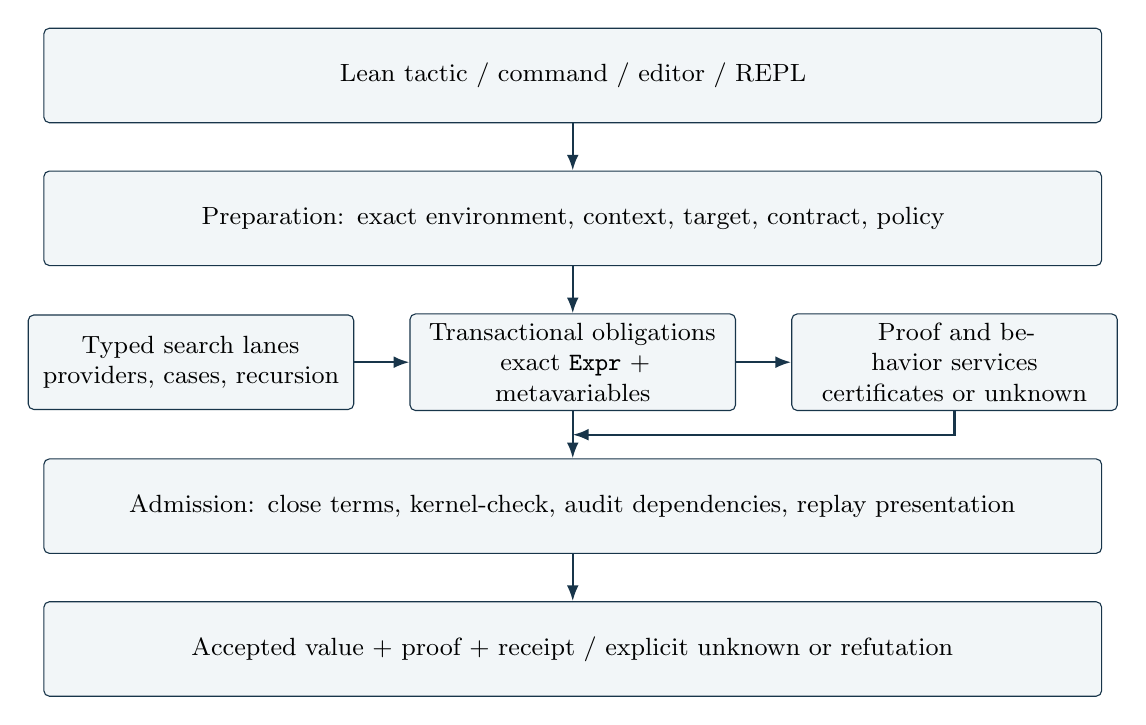
\begin{tikzpicture}[node distance=6mm and 7mm,
 box/.style={draw=Navy,rounded corners=2pt,fill=Pale,align=center,
   text width=39mm,minimum height=12mm,font=\small},
 wide/.style={box,text width=132mm},
 arrow/.style={-{Latex[length=2mm]},thick,draw=Navy}]
\node[wide] (front) {Lean tactic / command / editor / REPL};
\node[wide,below=of front] (prepare) {Preparation: exact environment, context, target, contract, policy};
\node[box,below=of prepare] (state) {Transactional obligations\\exact \texttt{Expr} + metavariables};
\node[box,left=of state] (plan) {Typed search lanes\\providers, cases, recursion};
\node[box,right=of state] (proof) {Proof and behavior services\\certificates or unknown};
\node[wide,below=of state] (admit) {Admission: close terms, kernel-check, audit dependencies, replay presentation};
\node[wide,below=of admit] (out) {Accepted value + proof + receipt / explicit unknown or refutation};
\draw[arrow] (front)--(prepare);\draw[arrow] (prepare)--(state);
\draw[arrow] (plan)--(state);\draw[arrow] (state)--(proof);
\draw[arrow] (proof.south) |- ([yshift=-3mm]state.south);
\draw[arrow] (state)--(admit);\draw[arrow] (admit)--(out);
\end{tikzpicture}
\caption{Proposed semantic architecture. Scheduler state and worker supervision surround the middle layer; no proposed term bypasses admission.}
\label{fig:architecture}
\end{figure}

The recommended module split is:

\begin{longtable}{@{}p{0.30\textwidth}p{0.64\textwidth}@{}}
\toprule Module & Responsibility \\
\midrule\endhead
\code{Leant2.Frontend} & Elaborate query syntax; expose tactic, command, and editor actions. \\
\code{Leant2.Query} & Immutable prepared query, environment lease, policies, and validated names. \\
\code{Leant2.MetaCompat} & Narrow version-specific wrapper around Lean elaboration, application, cases, projection, and declaration APIs. \\
\code{Leant2.Search.State} & Obligation dependency graph, branch snapshots, read/write footprints, and rollback. \\
\code{Leant2.Search.Scheduler} & Resumable lanes, priorities, cost layers, budgets, and cancellation. \\
\code{Leant2.Search.Structural} & Introductions, constructors, projections, local application, and dependent elimination. \\
\code{Leant2.Search.Library} & Provider indexing, retrieval, theorem adapters, and synthesis lemmas. \\
\code{Leant2.Search.Recursion} & Recursor templates, refinement carriers, call capabilities, and decreasingness obligations. \\
\code{Leant2.Proof} & Bounded proof services and explicit frozen-candidate verification. \\
\code{Leant2.Semantics} & Executable examples, certified abstractions, counterexample replay, and reversible buckets. \\
\code{Leant2.Admission} & Closure, checked declaration insertion, axiom and computability policy, and final receipt. \\
\code{Leant2.Worker} & Project-specific process protocol and environment lifecycle. \\
\code{Leant2.Controller} & Optional Lean REPL/editor service supervisor and durable command history. \\
\bottomrule
\end{longtable}

Only the small prototype in \code{lean/Leant2Core.lean} is implemented here.
This table is a proposed production layout, not a claim that these modules exist.

\subsection{Library first, worker second}

Inside a Lean proof, the current process already owns an appropriate environment
and local context. A tactic can invoke the semantic core directly, respecting
heartbeats, cancellation, and the outer elaborator's state. A standalone REPL
should instead use a replaceable worker built and launched under the target
project's toolchain. A globally compiled executable must not assume it can load
arbitrary incompatible \code{.olean} files.

The worker returns checked artifacts or process-local handles. Handles contain an
environment generation and become invalid after rollback, reset, import change,
or worker replacement. Durable state is source commands and checked artifact
metadata, not serialized raw pointer identities or orphaned metavariable IDs.
This preserves a useful operational boundary already identified in the repository
rewrite study.\cite{rewrite}

A hard timeout can terminate a worker even if cooperative Lean heartbeats do not
interrupt an external call or an unexpectedly expensive primitive. Every
external process has a separate budget and output limit. Stronger descriptor-bound
solver-launch policies may require a narrow platform shim; they are not necessary
to make the synthesis core Lean-native. The product should explicitly select
ordinary process isolation or the stronger policy rather than accidentally
weakening an existing guarantee.\cite{djexarch}

\subsection{A usable frontend}

The initial supported entrance should be ordinary Lean syntax:
\begin{lstlisting}
def choose : {f : ∀ A : Type, A → A → A //
    ∀ (A : Type) (x y : A), f A x y = y} := by
  leant2_core [] fuel 22 splits 0
\end{lstlisting}
This is implemented research syntax. A future \code{leant2} tactic should have a
small configuration object, explicit provider additions, contract mode, and a
way to expose alternatives. An exploratory \code{#synth} command can display a
candidate without adding it to the environment; an explicit accepted definition
commits it. Exact surface syntax for these future commands is not a semantic
commitment of this design.

The UI should show the inferred query, supported grammar, remaining proof
obligations, dependencies, and reasons for an unknown result. Useful diagnostics
include ``all candidates violate the supplied example,'' ``a decrease proof is
missing,'' and ``the target's universe constraints remain unresolved.'' A generic
``no solution'' is both less helpful and often logically wrong.

\section{Exact expressions and transactional search state}
\label{sec:state}

\subsection{Why an approximate neutral type language should not be authoritative}

Lean's expression language already represents universe parameters, dependent
function types, local constants, applications, projections, and binders. Its
metaprogramming framework provides the corresponding local and metavariable
contexts. The proposed core uses that representation rather than maintaining a
second approximate dependent type checker.\cite{metabook,applysource}

There is still a place for smaller representations. A propositional solver can
reify a formula; a length analysis can reify an arithmetic relation; a scheduler
can store a symbolic action plan. Such representations have \emph{local contracts}:
a result is interpreted back into an exact Lean obligation, and any theorem
claimed about that obligation is checked. No abstraction becomes the sole source
of a candidate's type, universe choices, or dictionary identity.

The earlier pure-IR proposal has real advantages: deterministic serialization,
explicit accounting, independent testing, and inexpensive structural operations.
The present design retains those advantages in the plan and indexing layer,
while avoiding the cost of reproducing Lean's dependent constraint semantics.
The tradeoff is tighter coupling to Lean metaprogramming APIs and more careful
state management. A \code{MetaCompat} facade and toolchain-pinned regression tests
are therefore architectural requirements, not optional maintenance work.

\subsection{The state owned by a branch}

A branch owns a root expression with holes, an ordered set of obligations, a
native metavariable state, a compatible local context, an environment lease,
branch-local semantic facts, and a continuation. Native universe metavariables
are as important as term metavariables. A constraint may couple two apparently
separate goals through a universe or an instance choice.

An obligation records its goal metavariable, role, dependencies, and policy:
\emph{program}, \emph{proof}, \emph{instance}, \emph{index equality},
\emph{termination}, or \emph{presentation replay}. These roles guide scheduling;
they do not introduce new logical judgments into Lean.

The dependency graph is not merely the syntactic occurrence relation between
targets. It includes metavariables occurring in local declaration types and
values, deferred constraints, instance arguments, and branch path conditions.
Read/write footprints are conservative over-approximations. False dependence
costs parallelism; missed dependence can corrupt branch composition.

\begin{proposition}[Sufficient condition for independent branch work]
Suppose two subsearches have disjoint writable metavariable closures, neither
reads an object the other can change, and their environment extensions and local
bindings are immutable or independently fresh. Then their successful assignments
can be combined without changing the result of either subsearch's recorded
checks, followed by ordinary final admission.
\end{proposition}
\begin{proof}
Each read in one subsearch observes the same expression and constraints before
and after applying the other's assignments. Fresh bindings do not capture or
identify existing bindings. Thus the recorded checked terms are unchanged under
composition of the assignments. Final admission remains necessary because the
footprint computation and branch implementation are not assumed correct by the
kernel.
\end{proof}

This is a sufficient engineering criterion, not an assertion that every pair of
Lean goals can be factorized. Existing work on factorized Lean proof states is
relevant, but synthesis additionally makes data witnesses and their behavior
share mutable unknowns.\cite{leantree}

\subsection{Algorithm 1: whole-continuation backtracking}
\label{sec:continuation}

The essential search operation is not ``solve this goal and return one term.''
It is ``solve these obligations and the continuation they constrain.''

\begin{lstlisting}[language={}]
search(state, obligations, continuation):
  if obligations are empty:
    return continuation(state)
  choose a ready obligation g
  for each admissible rule r for g:
    checkpoint := save branch state
    charge r to the non-rollback resource ledger
    outcome := run r transactionally
    if outcome produces subgoals:
      if search(updated state, subgoals ++ remaining, continuation) succeeds:
        return success
    restore checkpoint
  return unknown-or-exhausted-for-this-search
\end{lstlisting}

In the prototype, the remaining goal list is explicitly passed into each recursive
search call. A failed behavioral proof therefore restores the witness assignment
that produced it and tries another witness. Saving only the list of goal IDs
would be insufficient: those IDs can refer to changed metavariables.

\begin{example}[The first inhabitant is not necessarily the desired program]
For $A\to A\to A$, both projections are inhabitants. If the first projection is
committed immediately, the later constraint $f\ \mathsf{Nat}\ 11\ 29=29$ fails,
even though the second projection satisfies it. Joint backtracking recovers the
second projection. The prototype constructs that program and its proof.
\end{example}

A more subtle version appears in purely propositional search: a rule that assigns
a shared metavariable can make a sibling obligation unprovable. Thus the labels
``proof goal'' and ``safe tactic'' do not authorize arbitrary commitment. The
relevant invariant is preservation of the \emph{whole solution set under the
remaining constraints}, not merely local provability. Aesop's white-box design
is a useful starting point, but its inhabitation-oriented safe/unsafe distinction
must be interpreted carefully for joint program synthesis.\cite{aesop}

\subsection{What rollback does not roll back}

The search budget, cancellation token, worker deadline, telemetry counts, and
external-process accounting are outside branch snapshots. A branch that restores
a failed attempt has still consumed time and work. Otherwise cyclic search could
obtain unlimited resources by repeatedly rolling back its own accounting.

External effects are not transactional Lean state. Provider discovery may read
an immutable index; it must not import new modules or modify the user's environment
inside an ordinary choice point. Effectful proof plugins require an isolated
invocation boundary. Internal interruption and resource exceptions must escape
ordinary ``rule not applicable'' handlers.

\subsection{Protecting the caller and exporting a result}

An embedded tactic must establish which pre-existing metavariables it may assign.
The default is an ownership barrier: new synthesis holes are writable, outer
unknowns are rigid unless the user-facing tactic contract explicitly permits
assignment. Lean metavariable-depth mechanisms and a saved outer elaboration
state support this discipline. Merely rejecting unresolved variables at the end
does not prevent a search from having silently specialized its caller earlier.
\cite{metabook}

Before export, instantiate assigned holes; reject unresolved expression and
universe metavariables; abstract over the correct dependent local telescope;
retain universe parameters; verify the absence of dangling free variables; and
check the resulting declarations in a private environment. Raw expressions with
worker-local variable IDs never cross a durable boundary as self-contained proof
artifacts.

\section{Type-directed construction and dependent elimination}
\label{sec:structural}

\subsection{Focused introduction without losing behavioral alternatives}

For a target $\prod_{x:X}Y(x)$, introduce a fresh local $x:X$ and search for
$Y(x)$. Preserve the original binder information: explicit, implicit,
strict-implicit, or instance-implicit. This avoids making binding conventions an
accidental search restriction. Introduction is particularly effective for
higher-rank arguments because it exposes a quantified expected type before
choosing an implementation.

For a constructor target, enumerate constructors rather than committing to the
first one. In a product, dependent pair, or subtype, constructing one field can
change later field types. A data field is a choice point until every dependent
field and external contract has been satisfied. Proof irrelevance may justify
not enumerating multiple proofs of a \emph{fixed} proposition, but does not
justify merging different data fields or different assignments of a shared hole.

Normalization should be demand-driven. Compute weak-head normal form to expose
an outer function, inductive, or projection; avoid eagerly normalizing the full
target and the entire context at every node. Cache successful rigid reductions
with their transparency and environment settings. Reaching a reduction budget
is an unknown result for that operation, not a proof of disequality.

\subsection{Algorithm 2: dependent application with a telescope}

A provider may have type
\[
 c:\prod_{x_1:A_1}\prod_{x_2:A_2(x_1)}\cdots
       \prod_{x_k:A_k(x_1,\ldots,x_{k-1})}B(x_1,\ldots,x_k).
\]
Its arguments cannot be independently synthesized and later glued together.
The proposed application operation is:

\begin{enumerate}
\item Freshen the provider's universe parameters for this occurrence. Do not
reuse another occurrence's assignments because the printed name is the same.
\item Traverse the dependent telescope, creating appropriately scoped argument
holes and substituting each new hole into subsequent domains and the result.
\item Match the instantiated result against the target, recording residual
constraints. A rigid head mismatch can often reject cheaply; a flexible mismatch
may need an argument to be chosen first.
\item Identify determined parameters and delayed instance obligations. Schedule
remaining arguments and index equalities according to their dependency graph.
\item Search the entire continuation transactionally. Revisit earlier argument
choices when later domains, dictionaries, or the behavioral contract fail.
\end{enumerate}

Lean's application implementation already contains substantial logic for argument
creation, dependent-goal ordering, and repeated instance synthesis. Reuse it
behind the compatibility wrapper rather than copying a simplified approximation.
The prototype uses \code{MVarId.apply} with all new goals retained.
\cite{applysource}

Applying a polymorphic eliminator may not determine its result carrier. That is
a legitimate search obligation, not necessarily an error. The ordinary
application lane tries inference first; a separate carrier-invention lane
enumerates a bounded family of meaningful type expressions when inference alone
is insufficient. This division keeps simple synthesis fast without forbidding
higher-order constructions.

\subsection{Projections are first-class search actions}

Suppose
\[
 p:\sum_{n:\mathbb N}\operatorname{Fin}(n+1),\qquad
 \text{target }\operatorname{Fin}(p.1+1).
\]
The desired term is $p.2$. Applying the polymorphic constant \code{Sigma.snd}
to an entirely unknown pair first leaves too many unknowns: the return type
contains an unknown family and an unknown major premise. A result-directed
unifier need not reconstruct the intended pair from this information.

Instead, enumerate projections of already known structure values. Obtain
structure metadata from the environment, form the appropriate \code{Expr.proj}
with its known parent, infer its exact dependent type, and match that against
the target. Repeated projections can be explored at increasing cost; avoid
unbounded eager projection closure over recursive structures.

This was not merely a hypothetical issue. The expanded prototype initially
missed the Sigma projection example. A generic, metadata-driven local-projection
step made that example pass without changing its requested type or replacing it
with a reference implementation. The same action naturally exposes the value
and proof fields of a recursive subtype result.

\subsection{Dependent case analysis}

A case-split action chooses a local major premise and delegates dependent
elimination to Lean. Its result is a family of goals with branch-specific
contexts, substitutions, and equality information. The search must retain that
family as a single AND obligation, not accept a program that covers only the
branches easiest to solve.

For a vector type $\operatorname{Vec}(A,n)$, the query
\[
 \operatorname{Vec}(A,n+1)\to A
\]
permits a total head function. Dependent elimination removes the impossible empty
case and exposes an element in the cons case. The prototype exercises exactly
this indexed situation on a locally declared vector type, not a pre-existing
\code{head} function.

Index reasoning is also needed for transport:
\[
 n=m\ \to\ \operatorname{Vec}(A,n)\to\operatorname{Vec}(A,m).
\]
After equality elimination, the target becomes the source type. Some more
complicated index relations require explicit equalities, arithmetic proofs, and
transport terms. A search engine should not assume that all true index equalities
are definitional, or that swapping $n+m$ and $m+n$ is free.

An impossible branch must be eliminated by a valid recursor, constructor
no-confusion principle, or checked contradiction. Failure of a heuristic
unification attempt is not enough to erase a branch. Likewise, a proposition's
eliminator cannot be used to manufacture data in a sort prohibited by Lean's
elimination rules. The kernel boundary catches invalid proposals, but avoiding
such proposals is important for usable search.

\subsection{Local constants, lets, and expensive computations}

Retain local let values as well as their types. A let can expose information
useful for reduction while preserving a shared computation in the emitted
program. Unfolding a local let for matching does not require duplicating its
runtime work in the final source.

Search over let-bound reusable fragments should be a later, separate lane.
Naively introducing arbitrary lets recreates unrestricted term enumeration.
Useful triggers include a repeated expensive subtree, two obligations requiring
the same dictionary computation, or a recursive result whose value and proof are
both consumed. Candidate normalization must preserve sharing or account for its
loss in the quality metric.

\section{Universes, higher-rank types, and dictionary semantics}
\label{sec:universes}

\subsection{Universe constraints are native constraints}

A function polymorphic over \code{Type u} lives in the appropriate higher sort;
Lean's data universes are not Haskell-style impredicative types. Only the relevant
Lean rules determine whether a proposed type instantiation is legal. Leant2
should retain the original level expressions, including maxima and parameters,
and let Lean generate and solve level constraints.\cite{leanmanual,propositions}

In particular, do not lower a universe-polymorphic query to \code{Type 0} to make
it searchable and then present the result as a solution of the original query.
Such specialization can be an explicitly requested experiment, but it is a
different problem.

The prototype includes two independent universe-polymorphic callback arguments
and a result product across those universes. That example passed. It is a new
representative fixture, not the exact original two-universe benchmark recorded
as unresolved in the Leant repository. No acceptance of that original benchmark
is claimed here.\cite{indexing}

\subsection{A staged algorithm for polymorphic instantiation}

Use three levels of effort. First, infer arguments from a rigid target and known
provider arguments. Second, use expected-type-directed construction for
polymorphic arguments: when asked for $\forall X, X\to X$, introduce $X$ and its
argument rather than enumerating candidate monotypes. Third, when a type argument
remains genuinely underdetermined, propose a bounded type frontier built from
exact context types, target subexpressions, arrows, products, and certified
carrier templates.

Each proposal is a Lean expression checked at the provider's expected sort.
Correlated arguments share constraints, but separate provider occurrences do not
share fresh variables accidentally. Type-frontier depth, number of instantiations,
and generated expression size are observable resource limits. They are not
advertised as a rank restriction of Lean itself.

A nominal type alias may be unfolded for matching under the chosen transparency
policy, but retained identity matters to presentation, caching, and selected
instances. Types whose printed forms coincide under an abbreviated pretty-printer
must not be identified by their display strings.

\subsection{Instance synthesis is a service, not an erasure}

Lean instance synthesis already has its own rules for local instances, priorities,
input and output parameters, and postponement. Leant2 should use that mechanism
where the frontend requests ordinary Lean instance resolution.\cite{instances}
A delayed instance goal should wake when its input parameters become known;
repeatedly attempting it before anything changes wastes a search budget.

There are two distinct modes. In \emph{canonical instance mode}, normal Lean
resolution supplies omitted instance arguments. In \emph{explicit dictionary
search}, a data dictionary is an ordinary input or explicitly allowed candidate.
These modes must not silently interfere. Once a dictionary argument has been
chosen as data, another occurrence with the same class type is not interchangeable
unless equality or a suitable behavioral equivalence has been established.

For example, two values of \code{Inhabited Nat} may carry defaults 11 and 29.
A function constrained to return the second supplied default must retain which
dictionary was selected. The prototype has a behavioral regression for this
case. It uses an explicitly supplied dictionary projection and verifies the
observed value. This is materially different from checking that some instance
of \code{Inhabited Nat} was found.

Classes that are themselves propositions have proof-irrelevance properties;
classes carrying data generally do not. A global rule that merges all evidence
with the same class head would therefore be unsound as a behavioral search
optimization, even if every final term remained well-typed.

\section{Library reuse and proof services}
\label{sec:library}

\subsection{Provider discovery and indexing}

A practical synthesizer needs a large library without considering every constant
at every hole. Build an incremental index from accessible declarations. Its
primary keys include the normalized result head, explicit argument structure,
inductive family, proposition/data role, recursion shape, and coarse universe
shape. Maintain an unfiltered fallback lane for declarations whose result head
is flexible; an index is a proposal accelerator, not a proof that omitted
providers cannot work.

Local assumptions, constructors, projections, user-tagged synthesis lemmas, and
small trusted operation sets should be tried before broad environment retrieval.
A provider record contains the exact declaration name, universe parameters, full
type, visibility, computational classification, and provenance. Aliases can share
an underlying declaration without losing the frontend's chosen spelling.

A recommended user extension is a \emph{synthesis lemma}: a theorem or definition
that turns a desired construction into simpler subgoals. Its application is
ordinary Lean application and produces checked evidence. Tags additionally state
heuristic cost and a intended role, not unverified claims of logical safety.
Composition, traversals, folds, and container conversion lemmas are especially
valuable because they encode useful abstraction boundaries already present in
a library.

Learned premise ranking can improve the order of providers. It must operate on
the set of actually accessible declarations and remain optional. Retrieval-
augmented Lean proof systems provide relevant precedent; Leant2 should not
require a language model to obtain a working deterministic baseline.
\cite{leandojo}

\subsection{Proof obligations should use existing Lean automation}

Do not implement a second arithmetic prover merely to keep all search under one
name. The default proof service can progress through reflexivity and local
assumptions, controlled simplification, structural introduction, and small
rule-based search. Additional adapters can invoke \code{omega} for suitable
arithmetic goals, \code{grind} for its supported combination of reasoning
procedures, and Aesop with a query-specific rule set. Mathlib-dependent services
should be optional packages; the research prototype imports only \code{Lean}.
\cite{tactics,aesop}

Each invocation has its own step or heartbeat slice and the remaining global
deadline. A proof service returns a term, a proved negation, a residual obligation,
or unknown. A failed tactic invocation is not a negative theorem. Proof search
should use a narrow simplifier set when the contract depends on expensive
recursive definitions; uncontrolled unfolding can be much worse than the
original synthesis problem.

\subsection{Joint mode versus frozen verification}

During \emph{joint synthesis}, a proof can assign a program hole if the entire
assignment belongs to the same transaction. For instance, a reflexivity goal
$?m=n+1$ can determine a witness directly. The prototype's subtype-successor
example exploits this style of cooperation.

During \emph{candidate verification}, the proposed program is frozen. The proof
service may instantiate proof-local variables, but may not silently replace the
candidate or specialize its public type. Otherwise a receipt could describe one
candidate while proving a property of a different one. These two modes should
be different APIs, not a Boolean buried inside a generic solver.

Failure information also has scope. A proof of $\neg P(t)$ rejects $t$ for that
exact property in that exact context. It does not reject a different rendering,
a differently instantiated provider, or all terms sharing a type. A proof search
budget exhaustion supplies no such rejection evidence.

\subsection{Proof debt and early feasibility checks}

Allowing some unsolved proof obligations is essential: their types may depend on
future data choices. Allowing unlimited proof debt is equally dangerous: the
search can construct large programs whose obligations have no plausible path to
closure. Record a cost and readiness state for each obligation. After a specified
amount of program growth, give proof work a scheduler turn; wake index and
arithmetic obligations immediately after relevant assignments.

This is a ranking policy, not a sound pruning theorem. To preserve a fair mode,
branches with difficult obligations remain available in a separate cost layer.
A production heuristic mode may abandon them, but should report the policy and
budget that caused the loss.

\section{Certified recursion as the main expansion of capability}
\label{sec:recursion}

\subsection{Recursion should enter through a schema}

Most useful collection programs are not discovered efficiently by arbitrary
lambda-term enumeration. They reuse a fold, a structural recursor, a traversal,
or a well-founded recursion pattern. Leant2 should first search for an existing
combinator, then instantiate a certified scheme, and only later attempt more
ambitious recursion invention.

A scheme contains an eliminator or accepted recursive-definition template,
a result motive, typed branch holes, admissible recursive results, and proof
obligations. It exposes no unrestricted recursive constant. A branch can use a
recursive result only at the subterm and indices supplied by the recursor, or
through a call carrying a checked decrease proof.

For an inductive family, derive candidate schemes from Lean's inductive and
recursor metadata. Parameters, indices, mutual components, and recursive fields
must remain distinct. A prototype specialized to \code{List} is useful for
experiments but is not a general implementation for arbitrary inductive families.
Lean's own termination elaboration and recursor checks remain the final authority.
\cite{recursive}

\subsection{Algorithm 3: synthesize a result with its invariant}

Suppose the intended function is
\[
 f:D\to B,\qquad\forall x:D,\ R(x,f(x)).
\]
Instead of inventing $f$ and attempting an unrelated induction afterwards,
consider the dependent result type
\[
 F:\prod_{x:D}\{y:B\mid R(x,y)\}.
\]
For a structural branch with recursive field $x'$, the induction hypothesis
contains both $y':B$ and $h':R(x',y')$. This is precisely the information needed
to compose correctness locally.

\begin{lstlisting}[language={}]
refinementRecursion(query):
  recognize a structural input D and a candidate relation R
  construct motive M(x) := { y : B(x) // R(x,y) }
  ask Lean to instantiate a recursor or accepted equation template with M
  for each constructor branch:
    expose its fields and recursive results at M(smaller_input)
    synthesize the branch value and branch proof jointly
  close the recursor application
  project the implementation and its correctness theorem
  submit both declarations and all helpers to admission
\end{lstlisting}

The motive itself is a search choice. A relation may mention additional inputs,
an accumulator, or earlier choices. Generalize those inputs before induction
when the recursive step needs to change them. An induction hypothesis fixed at
the original accumulator is often too weak to justify a recursive call with a
new accumulator.

\subsection{Worked example: a map relation}

Let $\operatorname{MapRel}(g,xs,ys)$ be the inductive relation with rules
\[
 \frac{}{\operatorname{MapRel}(g,[],[])}\qquad
 \frac{\operatorname{MapRel}(g,xs,ys)}
 {\operatorname{MapRel}(g,x::xs,g(x)::ys)}.
\]
The intended output type is
\[
 (xs:\operatorname{List}A)\to
 \{ys:\operatorname{List}B\mid\operatorname{MapRel}(g,xs,ys)\}.
\]
The empty branch is immediate. In the cons branch, the recursive result gives
$ys$ and a proof of the premise of the second rule. That rule determines the
new head to be $g(x)$ and the new tail to be $ys$.

\begin{proposition}[The map relation specifies full elementwise behavior]
For every function $g$ and input list $xs$, there is exactly one list $ys$ such
that $\operatorname{MapRel}(g,xs,ys)$; its elements are the images of the elements
of $xs$ in the same order.
\end{proposition}
\begin{proof}
Induct on $xs$. At the empty list, the only applicable constructor produces the
empty output. At $x::xs$, an inversion of a relation proof forces the output to
be $g(x)::ys'$ and supplies the relation on $xs$. The induction hypothesis gives
existence and uniqueness of $ys'$, proving both claims.
\end{proof}

The separate Lean artifact \code{RecursionCertificates.lean} implements this
proof-carrying structural program. The schema and branch expressions are supplied
by hand in that artifact; it demonstrates the target certificate shape, not
automatic invention of the whole recursive program by the small prototype.

Contrast this relation with the weaker condition $|ys|=|xs|$. The latter can
permit a constant-filled output or a permutation, depending on available data.
A synthesizer should satisfy the actual contract, not guess that the user
intended map and silently substitute a stronger one.

\subsection{Recursive-call capabilities}

For structural recursion, the scheme's branch context gives named recursive
results only for the recursor's legitimate recursive arguments. For a function
with several changing parameters, a capability records the structurally smaller
argument together with the permitted generalized parameters.

For well-founded recursion, a capability has the schematic type
\[
 \prod_{y:D}\bigl(r(y,x)\to\{z:B(y)\mid R(y,z)\}\bigr),
\]
where $r$ has a supplied well-foundedness proof. The search may propose a call at
$y$, but it must also synthesize a proof of $r(y,x)$. A recursive name with an
unrestricted $D\to B$ type must never be available as an ordinary provider during
this construction.

The scheme guarantees totality only within the admitted Lean semantics and its
assumptions. Search itself may be implemented with \code{partial} metaprograms;
that does not make the generated recursive definitions partial. These are
separate functions with separate checking obligations.

\subsection{Algorithm 4: small, proof-checked measure search}

The initial well-founded lane should enumerate a deliberately limited grammar:
size of a data argument, a natural-number argument, a difference justified by a
branch bound, and lexicographic tuples of such measures. For each candidate
measure, generate the actual decrease goal for every proposed recursive call.
Use arithmetic or structural lemmas to prove it. Reject that measure if the
required proofs cannot be produced within its budget; do not report the desired
program impossible.

For a loop-like recursion that increments $i$ while $i<n$, $n-i$ is a natural
proposal. Because natural subtraction is truncated, a correct proof must use the
branch condition and the exact subtraction semantics. A template that reasons as
though natural subtraction were integer subtraction is not an acceptable
shortcut.

Mutual recursion may require a tagged sum state and a lexicographic measure.
Nested recursion may require stronger hypotheses or a different scheme. The
initial implementation should report these distinctions and offer a supplied
measure or skeleton as an extension point rather than hiding an unsupported case
behind arbitrary search failure.

\section{Inventing useful fold carriers and helper structure}
\label{sec:carriers}

\subsection{Backward demand explains function-valued carriers}

A fold result does not have to be the final scalar output. For indexing, the
fold can return a function that waits for the index. With a default value $d:A$,
let a Church-encoded list be instantiated at the carrier $\mathbb N\to A$.
The base and step are
\[
 b(i)=d,\qquad
 s(x,k)(i)=
 \begin{cases}x,&i=0,\\ k(j),&i=j+1.\end{cases}
\]
Then applying the resulting function to the requested index yields indexing with
a default. For an actual list encoding, correctness follows by induction on the
list and cases on the index. This statement is about encoded lists; it does not
assume a parametricity theorem characterizing every arbitrary inhabitant of a
Church type.

This example gives a concrete carrier-invention rule: when the final demand
still consumes an argument $I$ after an eliminator, try a carrier $I\to R$ before
forcing the eliminator to produce $R$ directly. A finite proposal grammar can
include $R$, $I\to R$, $S\times R$, and invariant-carrying dependent pairs,
where $I$ and $S$ come from exact context and target types.

The latest repository diagnostics already show that function-valued carriers and
an integer-case step can be found separately, yet fail to compose in the original
bounded indexing query. Thus carrier invention alone is not the entire repair.
Continuation-aware scheduling, context-sensitive ranking, and preservation of
pending obligations are equally important. This article does not claim to have
rerun or solved that exact legacy query.\cite{indexing}

\subsection{Algorithm 5: a carrier frontier}

Build the frontier from the demanded result type and the argument types of the
continuation. Generate candidate carriers in increasing structural cost, check
each at the eliminator's required sort, instantiate the eliminator, and attempt
its base and step jointly with the outer continuation. Memoize failed attempts
only under the full context, motive, and resource-bound key.

If the step can be synthesized in a reduced context, retain that result as a
candidate schema with explicit dependency parameters. Reintroduce it into the
original context through checked application. A failure in the reduced context
cannot justify pruning the full context, and a success there does not demonstrate
that the original whole query has been solved.

A useful abstraction is \emph{typed anti-unification}: replace differing,
well-scoped subexpressions in related demands by fresh parameters to propose a
shared helper type. Any resulting helper is ordinary Lean syntax and receives
its own synthesis and admission obligations. Anti-unification is a proposal
mechanism, not a proof that the helper suffices.

\subsection{Do not infer minimality from a heuristic score}

A compact carrier can create a complicated proof; an expanded carrier can make
correctness local and easy. Rank schemes by a vector containing program size,
number of recursive state components, estimated proof debt, and expected runtime
cost. The first accepted term is not automatically minimal under any of these
metrics. Claiming optimality requires a precisely defined cost, exhaustive lower
cost layers, and an admissible bound.

The natural initial objective is more modest: return a correct, readable
implementation quickly, preserve alternatives, and explain the chosen scheme.
User-supplied skeletons should remain first-class because they can turn a
research-level synthesis problem into small, independently checkable holes.

\section{Behavioral search, counterexamples, and abstraction}
\label{sec:behavior}

\subsection{Algorithm 6: certified counterexample-guided search}

For a universal contract $\forall x, R(x,t(x))$, maintain a set $T$ of validated
examples and an explicit candidate grammar. Candidate generation uses $T$ to
rank or restrict proposals. A verifier receives a frozen candidate and returns
one of three outcomes:
\[
 \mathsf{Proved}(p),\quad
 \mathsf{Counterexample}(x,q),\quad
 \mathsf{Unknown},
\]
where $q$ establishes the relevant violation for the exact candidate. With
preconditions, the counterexample includes evidence that the input is admissible.

\begin{lstlisting}[language={}]
repeat under a shared budget:
  obtain a candidate consistent with the current finite observations
  freeze and type-check the candidate
  run the universal proof service and counterexample service fairly
  if a proof of the entire contract is obtained: admit the result
  if a counterexample is validated:
    add it to T; refine buckets; update certified or heuristic pruning
  otherwise:
    retain the unresolved candidate, try alternatives, or report unknown
\end{lstlisting}

Executable tests can cheaply propose counterexamples. Under a strict evidence
policy, replay their exact violation in Lean before turning it into a certified
rejection. A test evaluator timeout is not a counterexample. A symbolic solver's
\code{sat} or \code{unsat} response is not, by itself, a Lean theorem.
The distinction is consistent with the existing project's replay-oriented
semantic boundaries.\cite{behavior,djexarch}

A finite input domain is special. Exhausting a complete enumeration together
with a proof of its coverage can establish a universal claim for that domain.
Enumerating lists only up to length four cannot prove a statement about all
lists; it can only help select a candidate whose full correctness is subsequently
proved.

\subsection{Observational equivalence must remain reversible}

For examples $T=\{x_1,\ldots,x_m\}$, define an observation vector
\[
 \operatorname{obs}_T(t)=(t(x_1),\ldots,t(x_m)).
\]
Equal vectors do not establish functional equality. They support a bucket of
currently indistinguishable candidates.

\begin{proposition}[Permanent merging can destroy a valid solution]
Even for total Boolean functions, keeping only one arbitrary representative of
each observation vector can remove the only candidate satisfying a later
observation.
\end{proposition}
\begin{proof}
Start with the test input \code{true} and candidates constant-true and identity.
Both return true. Keep constant-true and discard identity. Adding the input
\code{false} with required output false rejects the representative, although the
discarded identity function satisfies both tests.
\end{proof}

The local Python regression runs this exact counterexample. Keeping all
candidate derivations inside buckets allows refinement to split the bucket and
recover identity. A production implementation can store compact derivation DAGs
or regenerate discarded members, but must retain enough information to restore
them. Irreversible merging is legitimate only when a checked equality or a
suitable congruence theorem proves the replacement preserves every future
relevant observation.

For dependent expressions, even equality-based replacement may require
transporting later types. An equality cache cannot simply rewrite a raw subtree
without carrying the appropriate proof and context.

\subsection{Abstract semantics with explicit soundness direction}

Length, numeric intervals, constructor tags, finite maps, and algebraic shape
summaries can prune enormous families of programs. Each abstract domain should
provide a concretization relation and checked transfer laws. A useful invariant
is
\[
 \llbracket t\rrbracket\in\gamma(\widehat{\llbracket t\rrbracket}),
\]
with the notation adapted to the domain. An abstract impossibility result may
justify pruning only when this over-approximation and the relevant contradiction
are established under the exact query assumptions.

Under-approximations have a different role: they can produce witnesses or
counterexamples but cannot justify absence of all concrete solutions. Mixing the
two directions is a common source of unjustified negative claims. When an
abstract interpreter is merely an unproved heuristic, use its output for
ranking or report the loss of completeness explicitly; never label its pruning
certificate as a proof of the original Lean property.

Type-guided abstraction refinement and refinement-type synthesis provide strong
precedents for this organization. The Lean-specific change is that arbitrary
reconstruction obligations can be discharged in the same dependent type theory
as the target program. The architecture is not a claim to have invented
refinement types or counterexample-guided synthesis.\cite{synquid,tygar}

\subsection{Arithmetic and datatype translation traps}

An SMT adapter must explicitly distinguish unbounded integers, naturals with
nonnegativity constraints, truncated natural subtraction, machine integers,
and bitvectors with modular arithmetic. It must preserve defaults and failure
branches in operations modeled as total. Algebraic datatype encodings require
sound constructor and selector constraints; dependent indices require additional
invariants.

A counterexample generator for $i:\operatorname{Fin}(n)$ cannot independently
sample arbitrary $n$ and $i$ and forget the bound proof. More generally,
generation should follow the dependent telescope and produce well-typed inputs.
The exact tested instantiation, dictionaries, path conditions, and environment
belong in the replay record.

\subsection{Worked finite sketch experiment}

The supplied executable experiment searches 81 affine-fold sketches
\[
 F_{b,e,a,d}([])=b,\qquad
 F_{b,e,a,d}(x::xs)=e x+aF_{b,e,a,d}(xs)+d,
 \quad b,e,a,d\in\{0,1,2\}.
\]
It seeks list summation. A finite verifier enumerates the 121 lists of length at
most four over $\{0,1,2\}$. Counterexamples reduce the candidate set as follows:

\begin{table}[ht]\centering\small
\begin{tabular}{@{}cccc@{}}
\toprule Proposed $(b,e,a,d)$ & Candidates before check & Counterexample & Result \\
\midrule
$(0,0,0,0)$ & 81 & $[1]$ & Reject \\
$(0,0,0,1)$ & 11 & $[0]$ & Reject \\
$(0,1,0,0)$ & 5 & $[0,1]$ & Reject \\
$(0,1,1,0)$ & 1 & None in finite corpus & Submit for proof \\
\bottomrule
\end{tabular}
\caption{An executed finite-sketch experiment, not unrestricted recursive synthesis.}
\label{tab:cegis}
\end{table}

The selected sketch is subsequently proved in Lean to equal \code{List.sum}
for \emph{every} list of naturals. The proof is structural induction: the empty
case is reflexivity; the cons case simplifies the recurrence to $x+$ the
induction hypothesis. The checked theorem, not the 121 tests, supplies the
universal guarantee. The fold grammar itself was supplied, not automatically
invented.

\section{Scheduling, caching, and resource control}
\label{sec:scheduling}

\subsection{A portfolio with explicit progress units}

Use several resumable lanes rather than one monolithic priority queue: local
structural synthesis, library application, proof work, recursion schemes,
carrier invention, and finite sketches. A lane returns a candidate, a successor
state, a bounded progress event, or an explicit blocked/finished status. It must
not monopolize the system while trying to compute its next candidate.

A practical scheduler can reserve a fraction of turns for increasing-cost
exploration and use the remaining turns for heuristic priorities. A scoring
function might be
\[
 s(n)=w_1\,\operatorname{termSize}(n)+w_2\,\operatorname{newCases}(n)
       +w_3\,\operatorname{proofDebt}(n)+w_4\,\operatorname{providerCost}(n)
       -w_5\,\operatorname{progress}(n).
\]
These quantities are heuristic. Unless they are proved to be admissible lower
bounds for a specified objective, this is not an A* optimality argument.
Weights should be learned or tuned on a development set and exposed in the
receipt, not justified by a single successful example.

The scheduler should distinguish a failed candidate from a blocked state. A
blocked instance may become solvable when its type is known; a blocked proof may
become reflexive after a witness choice. Wake-up events are indexed by the
unknowns they depend on. Re-running every blocked solver after every assignment
would defeat the purpose of dependency tracking.

\subsection{Algorithm 7: fair exploration layers}

For an optional fair mode, give every action a positive structural cost and
explore bounds $k=0,1,2,\ldots$. At bound $k$, enumerate a finite library frontier,
finite type-carrier frontier, finite literal encodings, bounded scheme choices,
and bounded term/proof syntax. Increase both construction and checking budgets
by dovetailing. Deduplicate only by an equality or a replay-safe key that cannot
lose a semantically distinct branch.

Finite layers require care. A ``literal'' operation that can propose any natural
number in one unit of cost makes a layer infinite. Use a size-based encoding or
an explicitly finite literal set at each bound. A recursion scheme that invents
arbitrarily many auxiliary parameters has the same problem; its description size
must contribute to the layer cost.

The fast default may instead use beam limits and heuristic pruning. That is a
reasonable product choice, but its result is a bounded search result. Keeping
one fair reserve lane in a process with a hard deadline does not imply that every
solution is found before the deadline.

\subsection{Memoization requires more than the goal type}

A cache key should include the exact target, the ordered local-context signature,
reachable assignments and constraints, universe parameters, relevant dictionary
values, contract and example versions, provider/rule-set version, transparency
policy, environment generation, allowed axioms, and the searched resource bound.
An alpha-normalized representation may replace fresh local names with stable
positions, but the normalization must follow dependent binding structure.

Positive cache entries should be closed term schemas with explicit parameters,
not bare expressions containing old local IDs. They are instantiated and checked
in the new context. Negative entries should describe only the finite search
actually exhausted, unless accompanied by an appropriate refutation proof.

Two contexts containing variables printed as \code{x} need not refer to the same
variable. Two goals printed as \code{A} may use different universes. Two identical
function types may have different hard contracts. A cache indexed only by a
pretty-printed target will eventually mix such states.

\subsection{Learning reusable fragments}

Successful subterms can become candidate schemas with their dependency
parameters and proof certificates. Reuse is particularly attractive for fold
steps, dictionary transformations, and small dependent adapters. This is
\emph{library learning}, not permission to add an arbitrary theorem to the trusted
environment. Every learned helper is checked as an ordinary declaration.

During evaluation, learned fragments from the test problem must not enter other
baseline runs unless the experimental protocol explicitly permits online
learning. Source targets, equivalent aliases, and specification oracles must also
be excluded from the provider channel when the task is to synthesize rather
than retrieve the reference implementation.

\subsection{Memory and concurrency}

Native snapshots share persistent data, but retained branches can keep large
contexts and expression graphs alive. Store compact action traces for cold
branches, keep only a bounded working set of materialized snapshots, and
reconstruct a branch from the nearest checkpoint when revisited. Measure the
cost of reconstruction against the memory saved; no runtime advantage over the
existing Haskell implementation is established by the host language alone.

Parallel workers should operate on immutable prepared queries and independently
replayable plans. Do not merge arbitrary mutable native metavariable contexts
from different workers. Export a successful closed schema or a certificate, then
instantiate it in the receiving worker. Cancellation must propagate to proof
services, subprocesses, and queued continuations.

\section{Admission, trust, and executable meaning}
\label{sec:trust}

\subsection{Algorithm 8: the positive admission boundary}

Admission receives a completed candidate, contract proof, generated helper
declarations, and their provenance. It performs the following steps:

\begin{enumerate}
\item Check the environment lease and prepared-query identity. Reconstruct the
exact original type and contract rather than trusting a display string.
\item Instantiate assignments and close all expressions over the correct local
telescope and universe parameters. Reject dangling variables, unresolved holes,
and provisional helper references.
\item Insert helpers, the value declaration, and the correctness declaration into
a private environment through Lean's checked declaration path. Disallow
kernel-check bypass options, including \code{debug.skipKernelTC}.
\item Compute the transitive dependency closure of the accepted value and proof,
including helpers and referenced specifications. Enforce the query's axiom,
computability, safety, and provider policies.
\item Produce readable source. Re-elaborate that source under the recorded imports
and context, then check that it represents the intended result at the original
type and satisfies the original contract. Source replay is presentation evidence;
it never replaces the first kernel check.
\item Commit only after all checks pass. Attach a receipt identifying the query,
term, proof, dependencies, policies, source environment, and search status.
\end{enumerate}

An \code{inferType} call or successful unification alone is not the admission
boundary. The native kernel provides a checked declaration insertion API; its
use and version-specific wrappers should be verified against the pinned Lean
source.\cite{applysource,leanmanual}

\subsection{What the kernel guarantee does and does not say}

\begin{theorem}[Positive soundness relative to the admitted environment]
Assume that admission uses the intended Lean kernel with checking enabled, that
its accepted environment satisfies the stated dependency policy, and that it
accepts closed declarations corresponding to $t:A$ and $p:P(t)$. Then the
reported value has the requested type and the reported contract holds in that
Lean environment, independently of the search heuristics that proposed them.
\end{theorem}
\begin{proof}
Acceptance of the value declaration supplies the first typing judgment.
Acceptance of the correctness declaration supplies the second, referencing the
same admitted value. The environment and policy hypotheses make explicit the
assumptions under which those judgments are interpreted. No completeness,
ranking, abstract interpreter, or external solver is used in this deduction.
\end{proof}

The theorem is deliberately conditional on the actual kernel and environment.
An imported axiom of falsehood would make arbitrary contracts provable. A
dependency audit reports assumptions; it does not establish consistency of an
arbitrary user's axiom set. A production implementation should distinguish
standard Lean axioms, user-allowed axioms, and forbidden placeholders such as
\code{sorryAx}.

Kernel correctness is also not an unconditional guarantee about all compiled
external behavior. Unsafe implementations, external functions, and replacement
implementations can lie outside the pure logical model. Lean's recursive-
definition documentation explicitly distinguishes logical and executable
behavior for some facilities. An executable-mode policy needs a trustworthy
implementation boundary in addition to a logical theorem.\cite{recursive}

\subsection{Axiom and computability profiles}

A proof profile can permit \code{propext}, \code{Quot.sound},
and \code{Classical.choice}.
It always reports which were actually used. A stricter profile can demand an empty axiom
inventory. A program profile can permit standard logical reasoning in proofs
while disallowing noncomputable choice in the computational dependency path.
These are policies over the transitive dependency graph, not just a string search
in the emitted source.

Native evaluation shortcuts that introduce additional trusted axioms must not
be silently accepted under the strict kernel-reconstruction profile. Ordinary
\code{#eval} is useful as an observation, but is not itself a proof of a universal
property. The supplied tests use evaluation only for displayed outputs; proof
statements and axiom audits are separate.

An \code{IO A} term being well-typed does not prove it terminates, avoids unsafe
system calls, or produces a desired external trace. Effectful synthesis should
initially be restricted to explicitly permitted operation schemas with a
specified trace or state-transformer model. A weakest-precondition adapter can
be added later; general I/O behavior is outside the demonstrated prototype.

\subsection{Untrusted proposal services}

A learned model may propose a term, a skeleton, a measure, a library ranking, or
a proof. An SMT solver may propose coefficients or counterexamples. A heuristic
abstract interpreter may estimate infeasibility. All are useful, but none should
be able to mint an accepted-result value directly.

Keep capabilities for accepted candidates private to admission. A JSON object
with fields named \code{checked} or \code{proved} is not evidence. On worker
restart, previous process-local capabilities are invalid; durable artifacts are
rechecked before being treated as accepted in the new environment.

\section{What can be proved about the search itself?}
\label{sec:guarantees}

\subsection{Separate three different claims}

\emph{Sound acceptance} concerns whether returned results are valid.
\emph{Relative completeness} concerns whether a specified search eventually finds
a witness in a stated grammar. \emph{Practical coverage} concerns how often it
succeeds on representative workloads within a budget. They require different
evidence, and none follows simply from implementing the engine in Lean.

The prototype demonstrates positive results and rejection controls, not a
formal completeness theorem. The following propositions guide a future verified
small-grammar layer and describe conditions that the production scheduler must
not overstate.

\subsection{A finite grammar theorem}

\begin{definition}[Finite complete candidate set]
For a fixed query $Q$, let $C$ be a finite collection of fully specified value-and-
proof candidates, together with an enumeration containing every member. A checker
is \emph{decisive on $C$} when it terminates with accept or reject on every member,
and accepts exactly those members satisfying its specified admission predicate.
\end{definition}

\begin{proposition}[Finite exhaustion]
If the enumeration is complete, the checker is decisive on $C$, and all members
are rejected, then no member of $C$ satisfies the admission predicate. If one is
accepted, it is an admitted solution.
\end{proposition}
\begin{proof}
A satisfying member would occur in the enumeration and be accepted, contradicting
rejection of every member. The positive statement is the definition of the
checker's acceptance predicate.
\end{proof}

The hypothesis ``decisive'' is essential. A timeout does not count as rejection.
The conclusion concerns $C$, not every Lean term. A grammar with unresolved
metavariables is not a finite collection of completed candidates merely because
its printed sketch list is finite.

\subsection{Relative discovery under fair enumeration}

\begin{theorem}[Conditional eventual discovery]
Suppose a query has an admissible witness represented by a finite description in
an effectively enumerated grammar of completed candidates. Suppose that a fair
scheduler eventually runs that candidate with sufficient checking resources and
that its admission check succeeds in finite time. Then the scheduler eventually
discovers an admitted witness, provided no earlier heuristic operation
irreversibly removes it.
\end{theorem}
\begin{proof}
The witness has a finite position or cost in the effective enumeration. Fair
scheduling eventually reaches its description and a checking budget exceeding
its finite successful checking time. It is then accepted. Preservation of the
candidate prevents pruning from invalidating this argument.
\end{proof}

This is not a completeness theorem for Lean's ordinary unification procedure,
\code{apply}, Aesop, or the supplied depth-first prototype. They can miss terms
whose instantiations or intermediate structure they do not propose. A genuinely
complete fallback for a restricted grammar can enumerate fully explicit term
and proof syntax, including type and universe annotations, rather than depending
on an incomplete inference heuristic to reconstruct them.

Even such a fallback gives no finite-time decision procedure for arbitrary
inhabitation. It provides a precise conditional positive guarantee while the
fast lanes provide practical performance.

\subsection{Certified versus heuristic pruning}

A pruning step preserves the theorem above only when every removed candidate is
proved impossible for the exact remaining obligations, equivalent to a retained
candidate under all relevant continuations, or outside the advertised grammar.
Checking one example, merging by a pretty-printed type, or abandoning proof debt
does not meet that requirement.

A useful implementation convention is to attach a \emph{loss ledger} to every
query: beam truncation, incomplete provider retrieval, finite carrier frontier,
solver timeout, and unproved abstraction pruning are recorded separately. The
ledger is not itself a proof, but prevents the UI from turning a heuristic search
miss into a stronger mathematical statement.

\section{Implementation plan and realistic coverage}
\label{sec:roadmap}

\subsection{A staged implementation with acceptance gates}

\textbf{Stage A: exact core and admission.} Implement prepared queries, private
state transactions, local application, constructors, projections, and checked
result closure. Require regressions for scope capture, unresolved levels,
forbidden axioms, a false contract, and an exhausted inhabited goal. This stage
is close to the demonstrated prototype, except that production admission and
outer-metavariable ownership need stronger implementation than the research code.

\textbf{Stage B: practical library integration.} Add indexed provider retrieval,
dependent cases, dictionary modes, and bounded proof adapters. Gate on actual
project signatures across multiple universes and local instances; recheck emitted
source, not only in-memory expressions. Establish a compatibility matrix for
supported Lean versions.

\textbf{Stage C: contracts participate in search.} Introduce the obligation DAG,
explicit joint versus frozen modes, example caches, and cooperative scheduling.
Require the constrained-selector and dictionary examples to work without
committing the wrong first inhabitant. Add tests where a proof search assigns a
shared data unknown and must later backtrack.

\textbf{Stage D: certified recursive schemes.} Implement List, Nat, and a
representative indexed family first; then generalize via recursor metadata.
Require completed correctness statements for map-like relations, append,
folds, and safe indexing. Separate schema selection from arbitrary recursive
program invention in the public description.

\textbf{Stage E: counterexamples and abstractions.} Add reversible buckets,
dependent input generators, certified arithmetic/length translations, and finite
sketch solving. Require deliberate counterexamples to unsafe representative
merging and solver-model interpretation. No external solver response bypasses
Lean reconstruction.

\textbf{Stage F: carrier and measure invention.} Add function-valued and
invariant-carrying fold states, helper schemas, and limited well-founded measure
search. Gate each family on original, unchanged benchmark statements with
reference implementations excluded from the provider channel.

This is a dependency order rather than a calendar estimate. A stage is useful
on its own; the project need not wait for general recursion invention before
shipping practical dependent synthesis.

\subsection{Coverage by family}

\begin{table}[htbp]
\centering\small
\begin{tabularx}{\textwidth}{@{}p{0.24\textwidth}p{0.41\textwidth}Y@{}}
\toprule Family & Primary algorithm & Status in this package \\
\midrule
Polymorphic adapters & Introductions, local application, exact universes & Demonstrated by native synthesis \\
Products and sums & Constructors, known projections, cases & Demonstrated \\
Dependent composition and Sigma & Telescope application and dependent projections & Demonstrated \\
Indexed data and equality transport & Native dependent cases and equality elimination & Demonstrated on small fixtures \\
Data dictionaries & Explicit dictionary values plus canonical instance service & Demonstrated on two fixtures \\
Finite and universal selector contracts & Whole-continuation data/proof search & Demonstrated \\
Small arithmetic witnesses & Joint equality obligations, proof service & A successor witness demonstrated; broad arithmetic adapter planned \\
Collection traversals & Library reuse and certified structural recursion & Certificate shape demonstrated; generic synthesis planned \\
Higher-order fold carriers & Backward-demand carrier frontier & Algorithm specified, not implemented \\
Well-founded recursion & Measure grammar and decrease proofs & Algorithm specified, not implemented \\
Large algebraic proofs & Premise retrieval and domain proof services & Optional integration planned \\
Arbitrary effects / partiality & Explicit effect contracts and separate policy & Outside demonstrated core \\
\bottomrule
\end{tabularx}
\caption{Coverage goals and evidence levels for the supplied research package.}
\end{table}

No percentage of real-world Lean signatures is asserted. Coverage needs a defined
corpus, a provider policy, a specification policy, and a budget. A high pass rate
on easily inhabited types without discriminating behavior can greatly overstate
program-synthesis usefulness.

\subsection{Library choices}

Use Lean core metaprogramming and the standard library as mandatory dependencies.
Use Aesop as a bounded proof-search adapter rather than a replacement for the
program search state. Use \code{omega} and \code{grind} through the pinned Lean
interface. Put Mathlib-specific algebraic simplification, finite structures,
and domain lemmas in optional packages. Keep a small deterministic native test
suite that does not rely on importing the whole of Mathlib.\cite{tactics,aesop}

An SMT integration should start with a small theory and an explicit replay path,
not the ambition to translate arbitrary Lean propositions. Learned guidance is
best introduced after deterministic baselines and telemetry exist. The main
algorithms do not require a model server, and successful certificates remain
valid when the proposal service changes.

\section{Experiments and reproducibility}
\label{sec:experiments}

\subsection{What actually ran}

The working container had no Lean or Lake executable and its network requests
failed DNS resolution. The user-supplied tools documented AXLE's remote check
endpoint. A Wolfram Language HTTP client successfully submitted Lean source to
that endpoint with environment \code{lean-4.34.0},
\code{ignore_imports = false}, and \code{theorems_only = false}.
Both final successful runs reported Lean 4.34.0 or the matching environment.
The API and its check options are publicly documented.\cite{axle}

The final compilation inputs are these standalone files:
\begin{quote}
\code{lean/Validation.lean}\\
\code{lean/RecursionCertificates.lean}
\end{quote}
The former is a comment-stripped,
blank-line-stripped version of the readable core plus tests, not a different
algorithm. The local and remotely reported SHA-256 values match. The service
appended one terminal newline in its echoed content; it did not change the
import header. The Python checker accepts only exact echo or that one explicitly harmless
transformation, not arbitrary source rewriting.

The receipts contain compact transcriptions of observed tool responses and
source identities, rather than a claim that a local \code{lake build} ran.
The service identifies its executor build and environment but does not report
a Mathlib commit. The sources explicitly import \code{Lean}; the service's
advisories about its preferred Mathlib header are retained as advisories, not
silently suppressed.

\subsection{Native synthesis results}

\begin{table}[ht]\centering\small
\begin{tabularx}{\textwidth}{@{}Yrr@{}}
\toprule Category & Number & Passed \\
\midrule
Polymorphic identity/composition/substitution & 3 & 3 \\
Product, sum, and empty-type constructions & 4 & 4 \\
Dependent composition, Sigma, indexed head, transport & 5 & 5 \\
Higher-rank and two-universe callbacks & 2 & 2 \\
Contextual default and explicit dictionary selection & 2 & 2 \\
Behaviorally constrained value synthesis & 3 & 3 \\
Conjunction and disjunction proofs & 2 & 2 \\
\midrule
Synthesis declarations & 21 & 21 \\
Expected-failure and exhaustion controls & 4 & 4 \\
Additional statements about outputs & 8 & 8 \\
\bottomrule
\end{tabularx}
\caption{Executed research fixtures. These are not a representative performance benchmark.}
\label{tab:tests}
\end{table}

The native run is identified by request
\code{3ae6e8d8-a4a5-491a-a01a-1883ff4b35c1}. It returned no failed declarations,
no Lean errors, and no Lean warnings. The explicit audit covered all 21 synthesis
declarations and four controls. Of those 25 inventories, 24 were empty; the
indexed-head declaration used \code{propext}. None used \code{sorryAx},
\code{Classical.choice}, or \code{Quot.sound}.

The controls require failure on \code{False}, a false subtype contract, an
uninhabited polymorphic choice signature, and \code{Nat} with zero search fuel.
The last control is especially important: failure on an inhabited type must not
be interpreted as a refutation. A \code{fail_if_success} control demonstrates
that the invocation failed; it does not prove a general classification theorem
for every possible failure path.

The prototype is approximately a hundred lines of search and tactic integration,
plus documentation and tests. It implements bounded depth-first search, not the
portfolio scheduler, production cache, complete type-carrier frontier, or
recursion invention proposed above. It delegates finished declarations to the
ordinary Lean compiler. Its explicit audit is in the test file, not a complete
production admission subsystem.

\subsection{The projection regression and the axiom audit}

The first expanded run missed the dependent Sigma projection. The correction was
not to add the desired whole solution as a provider, but to enumerate projections
of known local structures before attempting generic provider application. This
is a small example of a general design principle: when an eliminator's result
depends on its major premise, choose the known major premise before matching the
result.

A later run successfully constructed all synthesis declarations but failed an
initially over-strict empty-axiom audit. Native indexed elimination had introduced
\code{propext}. The final audit permits the documented standard Lean axioms and
prints each actual inventory. The report therefore does not describe that result
as axiom-free. Failed development attempts and their request IDs are retained in
\code{receipts/development-notes.md}.

\subsection{Recursion and finite-sketch results}

The recursion run is identified by request
\code{7593e833-ccb3-40da-ae93-689c27d941a3}. It validates a proof-carrying map,
the affine-fold template, the universal sum theorem, and a proof of emptiness
for polymorphic choice. The map, template, and emptiness proof have empty axiom
inventories. The sum theorem uses only \code{propext}.

The local Python model selected $(0,1,1,0)$ from 81 fold sketches and exercised
121 finite inputs in the verifier. Its full trace is recorded in
\code{experiments/results.json}. The second model demonstrates that destructive
observational merging loses identity on the two Boolean inputs, whereas retained
derivations recover it. These experiments test precise invariants; their tiny
search spaces do not substantiate a speed claim for a large Lean project.

\subsection{How to reproduce}

From the package root, the following commands identify the intended workflow:
\begin{lstlisting}[language={}]
python tools/verify_package.py
python experiments/search_models.py
# With Lean 4.34.0 installed:
lean lean/Validation.lean
lean lean/RecursionCertificates.lean
# Or remote checking, requiring network access:
python tools/check_lean.py lean/Validation.lean --audit-marker LEANT2_AUDIT:
python tools/check_lean.py lean/RecursionCertificates.lean \
  --audit-marker LEANT2_RECURSION_AUDIT:
# Build the article:
cd article
latexmk -pdf Leant2.tex
\end{lstlisting}

A \code{lean-toolchain} file pins the requested version. The remote checker writes
a fresh full JSON receipt and validates errors, incomplete declarations, sorry
warnings, the audit marker, and the source echo. It does not use \code{okay=true}
alone as evidence. The readable split modules are provided for development; the
standalone validation file avoids any ambiguity about module search paths in a
remote request.

\section{Evaluation design for a production Leant2}
\label{sec:evaluation}

\subsection{Build a corpus that measures synthesis, not easy inhabitation}

A serious evaluation should contain exact statements from standard-library and
project code, grouped by the family in Section~\ref{sec:roadmap}. For each query,
record its imports, target type, hard contract, examples, permitted providers,
axiom/computability policy, and resource limits. Preserve original binder order,
universes, dictionaries, and default-bearing behavior.

Exclude the target definition, aliases of it, and known reference implementations
from synthesis retrieval. Specification symbols are allowed to describe the
problem but are not automatically construction providers. A proof theorem can
also leak a reference implementation through a witness or an equality; dependency
inspection should identify such leakage. Maintain separate training/development
and held-out sets, including tasks whose useful providers were not selected in
tuning. Retrieval research in Lean highlights the importance of accessible
premises and meaningful data splits.\cite{leandojo}

Include deliberately weak specifications to measure ambiguity, and deliberately
false contracts to exercise actual rejection rather than mere lack of candidate
production. A negative control that never reaches a verifier demonstrates much
less than one that checks and rejects an incorrect candidate.

\subsection{Baselines and ablations}

Compare against local exact/assumption and library-application baselines,
configured Aesop and domain tactics, a post-filter-only variant of the same
candidate generator, and the existing Leant/Djex pipeline on the exact shared
fragment. Use a separate table for goals that the older frontend cannot express
without approximation. Do not count a richer frontend as a speed improvement on
a different problem.

Ablate whole-continuation rollback, known-major projections, dependent carrier
search, proof-carrying recursion, context-sensitive caching, and reversible
buckets. Preserve the same grammar and budget when possible. For a component
that expands the grammar, report that expansion separately from search ordering.

Report accepted solutions with proofs, proved counterexamples, unresolved
candidates, unsupported operations, and search losses. Measure candidate visits,
proof work, normalization work, maximum retained state, kernel-check cost,
source-replay cost, and end-to-end latency. Cold setup and warm query processing
should be distinguished. Use repeated runs for timing claims and record cache
hits explicitly.

\subsection{Code quality and maintainability}

Correctness is necessary but not sufficient for generated code to be useful.
Measure source size, recursion shape, dependency footprint, explicit casts,
unnecessary classical reasoning, sharing of expensive computations, and clarity
of local names. Let the user choose between a compact combinator expression and
a readable equation-style definition, provided both replay successfully.

Do not optimize only for a small proof term while emitting an exponential
algorithm. Conversely, do not discard a straightforward total implementation
because its source contains a few more lines than an opaque helper call.
Resource-aware synthesis has studied formal cost specifications; a future
Leant2 cost model should build on that idea with an explicitly validated
connection to its chosen Lean execution model.\cite{resources}

\section{Conclusions}

Leant2 is most promising as a \emph{proof-carrying construction system}, not as
a new approximate type language wrapped around Lean replay. Its central data
structures should retain exact Lean binding and dependency information; its
search should treat values and their behavior as one backtrackable problem; and
its recursion support should expose only justified recursive results and calls.

The native experiments show that a small amount of Lean metaprogramming already
handles useful polymorphic, dependent, indexed, and behavioral tasks. They also
expose a real search issue---dependent projection from a known parent---and make
its generic correction testable. The larger proposed capabilities are concrete
algorithms with clear acceptance boundaries, but remain implementation work.

The recommended first release combines exact local synthesis, provider reuse,
dependent cases, controlled proof services, honest results, and robust admission.
The next expansion should be invariant-carrying recursion and carrier invention.
Counterexamples, abstraction, learned guidance, and large-library retrieval then
become cooperating proposal mechanisms, not alternative sources of truth.

\appendix
\section{Proposed internal interfaces and invariants}
\label{app:interfaces}

The following is architectural pseudocode, not compiled Lean API declarations:
\begin{lstlisting}[language={}]
PreparedQuery:
  immutable environment lease
  original local telescope, target, contract
  provider inventory and rule-set versions
  grammar, trust policy, computational policy, budgets

SearchBranch:
  native branch snapshot + explicit action plan
  root candidate expression
  obligation dependency graph
  branch-local constraints and semantic observations
  continuation and heuristic score

ProofService.checkFrozen(candidate, proposition, budget):
  Proved(proof) | Disproved(proofOfNegation) | Unknown(reason)

Rule.expand(branch, obligation, quantum):
  Yield(successor) | Blocked(dependencies) | Finished(status)

Admission.check(preparedQuery, candidate, proof, helpers):
  Accepted(closedArtifact, receipt) | Rejected(diagnostic)
\end{lstlisting}

A candidate's type is the exact \code{Expr} from the prepared query, not a second
recursive type representation. A rule may propose an expression with new holes
but cannot construct an accepted-result capability. A proof service in frozen
mode cannot assign program holes. A snapshot's lease must match the environment
in which it is restored. A cache hit is checked in the receiving context.
A budget is never restored by branch rollback.

For a production implementation, add explicit invariant tests for context
abstraction, universe freshness, dictionary identity, interrupt propagation,
false contracts, proof-service assignments, and source replay. Fuzz small typed
contexts and compare accepted expressions with independent kernel insertion.
An optimization may remove a branch only under a declared evidence rule or an
explicit loss-of-completeness policy.

\section{A short reading guide to the supplied code}
\label{app:code}

\code{lean/Leant2Core.lean} contains the research tactic. The \code{transaction}
function saves native state and restores failed attempts. The recursive
\code{search} function passes the complete remaining goal list through every
alternative. It introduces function binders, enumerates local terms and
projections, tries providers and target constructors, and optionally performs
bounded case analysis. It rejects unresolved metavariables before returning.

The code intentionally favors inspectability over asymptotic performance. It
rescans local context and has no sophisticated provider index. Its fuel is a
bound on explored derivation depth along each recursive path, not a strict global
node-count budget. Global Lean heartbeats bound additional work. Reusing the
same \code{splits} allowance in restored alternatives is appropriate for a
per-derivation bound, but must not be confused with the production non-rollback
work ledger described in Section~\ref{sec:state}.

\code{lean/Tests.lean} contains the readable test module. Its tests do not import
reference implementations of the requested adapters. The only explicitly named
providers are a dependent projection, a class projection, and the supplied
dictionary accessor. Target constructors and \code{Eq.refl} are discovered or
added by the search. The controls restore the surrounding proof state using
Lean's testing tactic behavior.

\code{lean/Validation.lean} is the exact remote compilation input, generated by
joining the core and tests and removing comments and blank lines. It is not a
second independently maintained engine. \code{tools/verify_package.py} checks
that relationship and the source identities in the receipts.

\code{lean/RecursionCertificates.lean} illustrates the intended shape of
recursive results and gives the universal certificate for the independently
selected affine-fold parameters. It should not be presented as a demonstration
that \code{leant2_core} invents recursion.

\section{Source inventory and baseline boundaries}
\label{app:sources}

The repository review used the current README files, Djex's architectural guide,
Leant's behavioral-synthesis guide, the existing Lean-rewrite study, and the
14 September indexing/composition diagnostic. It did not execute either legacy
repository's build or benchmark suite. The references below identify pinned
source documents whenever possible. The existing rewrite study itself describes
older snapshots; this article does not substitute those old snapshots for the
current baseline.

The API compatibility check used Lean 4.34.0's application implementation and
live remote \code{#check} probes. The current reference manual supplied the
semantics of propositions, recursion, and proof tactics. Literature on
refinement synthesis, type-guided abstraction, white-box proof search, and
premise retrieval supplies context for the proposed combination of algorithms.
The article does not claim novelty for those established techniques.

The package has no generated checksum-list files. Source digests are part of
verification receipts because they identify the exact remotely submitted inputs.
No font files, external repository copies, or hidden credentials are included.

\begin{thebibliography}{99}
\bibitem{leant}
Vladimir Reshetnikov and contributors.
\emph{Leant repository}, README at commit
\code{6bf05ad78c467989e68290f2d08bbed40802d485}.
\url{https://github.com/VladimirReshetnikov/Leant/blob/6bf05ad78c467989e68290f2d08bbed40802d485/README.md}.

\bibitem{djex}
Vladimir Reshetnikov and contributors.
\emph{Djex repository}, README at commit
\code{e8778f4ebd63e1f9b9b410fa4de8d14a8a04c9e5}.
\url{https://github.com/VladimirReshetnikov/Djex/blob/e8778f4ebd63e1f9b9b410fa4de8d14a8a04c9e5/README.md}.

\bibitem{djexarch}
Djex project. \emph{Djex architecture}, source architecture guide, inspected at
the Djex commit above.
\url{https://github.com/VladimirReshetnikov/Djex/blob/e8778f4ebd63e1f9b9b410fa4de8d14a8a04c9e5/docs/architecture.md}.

\bibitem{behavior}
Leant project. \emph{Behavioral assertions during synthesis}, inspected at the
Leant commit above.
\url{https://github.com/VladimirReshetnikov/Leant/blob/6bf05ad78c467989e68290f2d08bbed40802d485/docs/behavioral-synthesis.md}.

\bibitem{rewrite}
Leant project. \emph{Rewriting Leant and Djex in Lean 4: Feasibility,
Architectural Consequences, Tradeoffs, and Recommended End State}.
Repository report dated 15 August 2026; inspected as a prior design, not a new
contribution of this article.
\url{https://github.com/VladimirReshetnikov/Leant/blob/6bf05ad78c467989e68290f2d08bbed40802d485/docs/Leant_Djex_Lean4_Rewrite_Analysis/Leant_Djex_Lean4_Rewrite_Analysis.tex}.

\bibitem{indexing}
Djex project. \emph{Indexing-composition diagnostics}, recorded in commit
\code{e8778f4ebd63e1f9b9b410fa4de8d14a8a04c9e5}, 14 September 2026.
\url{https://github.com/VladimirReshetnikov/Djex/commit/e8778f4ebd63e1f9b9b410fa4de8d14a8a04c9e5}.

\bibitem{leanmanual}
Lean Focused Research Organization and contributors.
\emph{The Lean Language Reference}, version identified as 4.34.0 when accessed
17 September 2026.
\url{https://lean-lang.org/doc/reference/latest/}.

\bibitem{metabook}
Lean community. \emph{Metaprogramming in Lean 4}, chapter ``MetaM.''
\url{https://leanprover-community.github.io/lean4-metaprogramming-book/main/04_metam.html}.

\bibitem{applysource}
Lean contributors. \emph{Lean 4.34.0 source: Meta tactic application}.
\url{https://github.com/leanprover/lean4/blob/v4.34.0/src/Lean/Meta/Tactic/Apply.lean}.

\bibitem{propositions}
Lean Language Reference. \emph{Propositions}.
\url{https://lean-lang.org/doc/reference/latest/The-Type-System/Propositions/}.

\bibitem{recursive}
Lean Language Reference. \emph{Recursive Definitions}.
\url{https://lean-lang.org/doc/reference/latest/Definitions/Recursive-Definitions/}.

\bibitem{instances}
Lean Language Reference. \emph{Instance Synthesis}.
\url{https://lean-lang.org/doc/reference/latest/Type-Classes/Instance-Synthesis/}.

\bibitem{tactics}
Lean Language Reference. \emph{Tactic Reference}.
\url{https://lean-lang.org/doc/reference/latest/Tactic-Proofs/Tactic-Reference/}.

\bibitem{synquid}
Nadia Polikarpova, Ivan Kuraj, and Armando Solar-Lezama.
\emph{Program Synthesis from Polymorphic Refinement Types}.
PLDI 2016; arXiv:1510.08419.
\url{https://arxiv.org/abs/1510.08419}.

\bibitem{tygar}
Zheng Guo, Michael James, David Justo, Jiaxiao Zhou, Ziteng Wang,
Ranjit Jhala, and Nadia Polikarpova.
\emph{Program Synthesis by Type-Guided Abstraction Refinement}.
arXiv:1911.04091, 2019.
\url{https://arxiv.org/abs/1911.04091}.

\bibitem{aesop}
Jannis Limperg and Asta Halkj{\ae}r From.
\emph{Aesop: White-Box Best-First Proof Search for Lean}. CPP 2023.
Implementation and rule-set documentation:
\url{https://github.com/leanprover-community/aesop}.

\bibitem{leantree}
Mat\v{e}j Kripner, Michal \v{S}ustr, and Milan Straka.
\emph{LeanTree: Accelerating White-Box Proof Search with Factorized States in
Lean 4}. arXiv:2507.14722, 2025.
\url{https://arxiv.org/abs/2507.14722}.

\bibitem{leandojo}
Kaiyu Yang et al.
\emph{LeanDojo: Theorem Proving with Retrieval-Augmented Language Models}.
arXiv:2306.15626, 2023.
\url{https://arxiv.org/abs/2306.15626}.

\bibitem{resources}
Tristan Knoth, Di Wang, Nadia Polikarpova, and Jan Hoffmann.
\emph{Resource-Guided Program Synthesis}. PLDI 2019; arXiv:1904.07415.
\url{https://arxiv.org/abs/1904.07415}.

\bibitem{axle}
Axiom Math. \emph{AXLE documentation: Check}.
\url{https://axle.axiommath.ai/v1/docs/tools/check/}.
Accessed 17 September 2026. Remote clients were adapted from the workflow
described in the user-supplied \code{tools.zip}.
\end{thebibliography}
\end{document}
